\documentclass[10pt,a4paper]{article}
\usepackage[utf8]{inputenc}
\usepackage{amsmath}
\usepackage{amsfonts}
\usepackage{amssymb}
\usepackage{geometry}
\usepackage{verbatim}
\usepackage{enumerate}
\usepackage{fancyvrb}
\usepackage{graphicx}
\usepackage{hyperref}
\usepackage{tikz}
\usetikzlibrary{positioning}
\usetikzlibrary{shapes,snakes}
\usepackage[english]{babel}

\geometry{legalpaper, margin=1.5in}

\author{William Schultz}
\begin{document}
\title{Weakest Preconditions}
\author{William Schultz}
\maketitle

The notion of \textit{weakest precondition} in program analysis derives from the work of Dijkstra \cite{1975dijkstrawp}. He introduced the \textit{Guarded Command Language} as a simple modeling language for program specification e.g.
\begin{center}
    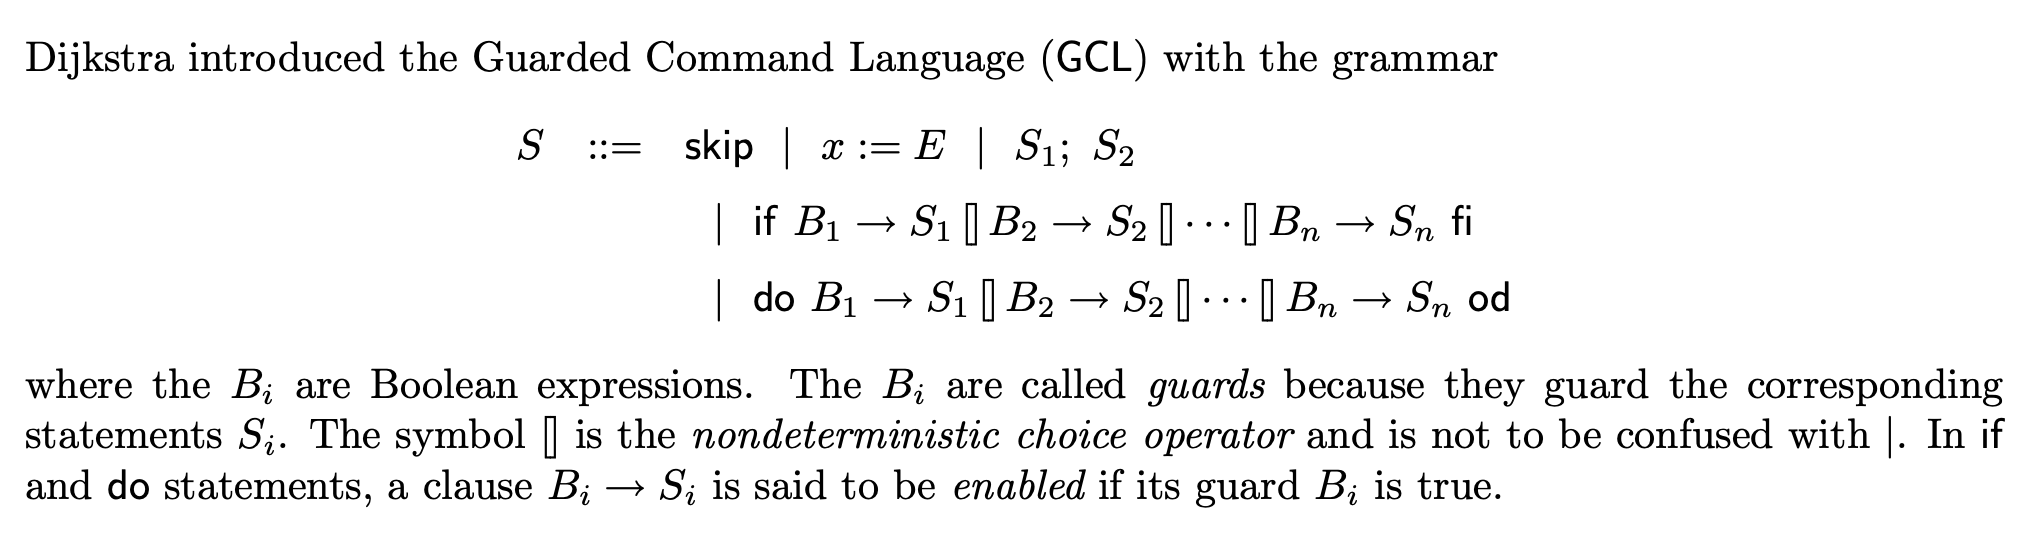
\includegraphics[scale=0.3]{gcl_grammar.png}
\end{center}
So, given a program $S$ and a postcondition $\varphi$, we define the \textit{weakest precondition} as the weakest property of the input state that guarantees that $S$ will terminate with the postcondition $\varphi$, denoted $wp(S, \varphi)$. In the definition of GCL, we can provide definitions of how to compute the weakest precondition for various program statements. For example, for an assignment statement $x := E$, we have that
\begin{align*}
    wp(x := E, \varphi) \equiv \varphi\{E/x\} \\
\end{align*}
where $\varphi\{E/x\}$ represents the property $\varphi$ with apperances of $x$ in $\varphi$ replaced with $E$. For example,
\begin{align*}
    wp(x := x + 1, x = 3) &\equiv (x = 3)\{x+1/x\} \\
    & \equiv (x+1) = 3\\
    & \equiv x = 2\\
\end{align*}


\bibliographystyle{plain}
\bibliography{../../references.bib}

\end{document}